\section{Evaluation}

\begin{frame}{$\SPSER$ transactional memory}
  Key algorithmic features:
  \begin{itemize}
  \item single version
  \item lock-based
  \item lazy snapshot
    \begin{itemize}
    \item[] when executing $r_i(x_j)$
    \item[] if $\clockOf{T_j} > \clockOf{T_i}$ then
    \item[] \hspace{1em} revalidate prior reads
    \end{itemize}        
  \item at commit time, $\clockOf{T_i} = \max \{ \clockOf{T_j} : T_i \depends T_j \} + 1$
  \end{itemize}
\end{frame}

\begin{frame}{Evaluation parameters}
  \begin{itemize}
  \item open-source C implementation (based on TinySTM)
  \item comparison with TinySTM (v1.0.5)
  \item TinySTM applications suite (bank, linked-list, red-black tree)
  \item AMD Opteron48
    \begin{itemize}
    \item a 48-cores machine with 256 GB of RAM.
    \item 4 dodeca-core AMD Opteron 6172 (8 NUMA nodes)
    \end{itemize}    
  \end{itemize}
\end{frame}

\begin{frame}{Bank benchmark}
  \begin{figure}
    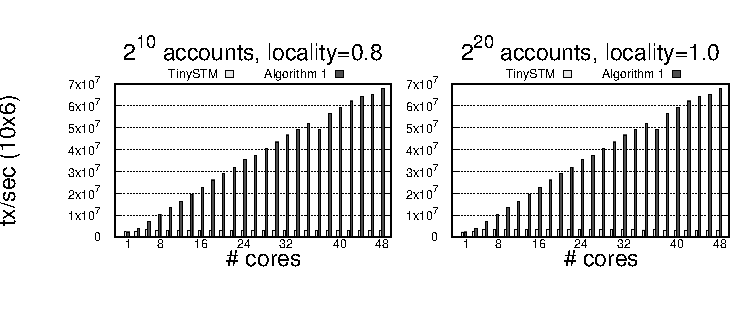
\includegraphics[scale = 0.8]{results/intset/bank.pdf}
  \end{figure}
  Each account belongs to a branch.\\
  Locality = likeliness to pick an account in the thread-local branch.\\
  \smallskip
  In the above figure, Locality set to $0.8$ \\
\end{frame}
  
\begin{frame}{Bank benchmark}
  \begin{figure}
    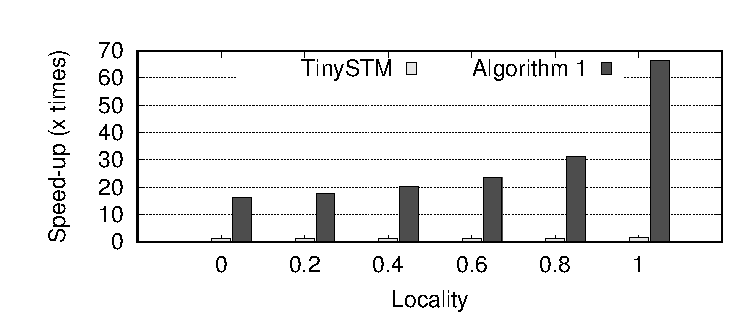
\includegraphics[scale = 0.8]{results/bank-speedup/bank-speedup.pdf}
  \end{figure}
  Varying locality, using $48$ threads
\end{frame}

\begin{frame}{Other benchmarks}
  \begin{figure}
    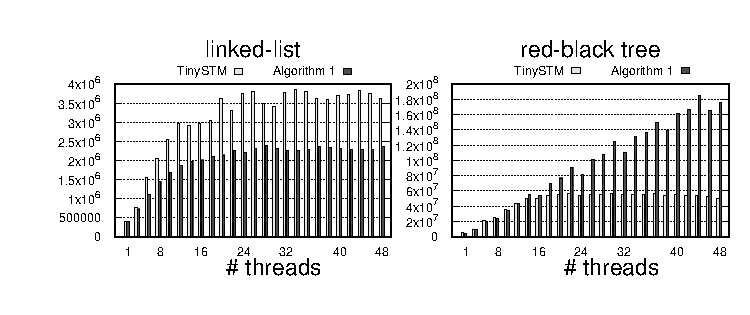
\includegraphics[scale = 0.9]{results/intset/ll-rb.pdf}
  \end{figure}
  linked-list = randomly add/remove $x \in [-255,255]$ \\
  red-black tree = randomly add/remove $x \in [0,10^7]$ 
\end{frame}
